\documentclass[11pt, oneside]{article} 
\usepackage{geometry}
\geometry{letterpaper} 
\usepackage{graphicx}
	
\usepackage{amssymb}
\usepackage{amsmath}
\usepackage{parskip}
\usepackage{color}
\usepackage{hyperref}

\graphicspath{{/Users/telliott/Github/calculus_book/png/}}
% \begin{center} 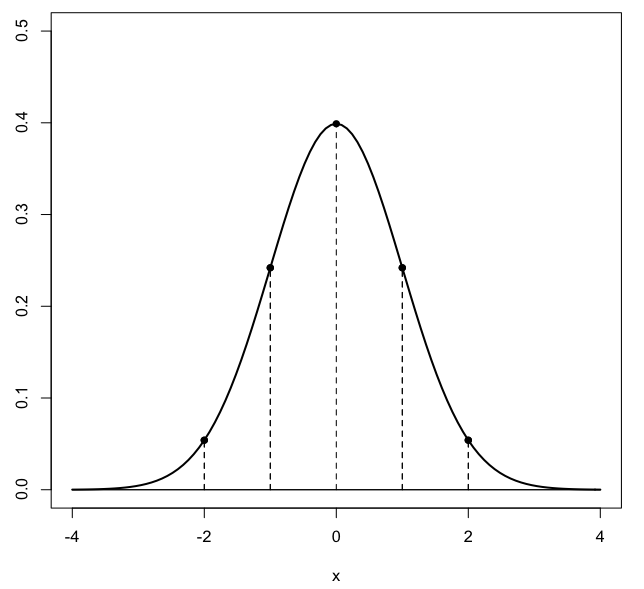
\includegraphics [scale=0.4] {gauss3.png} \end{center}

\title{Analytic geometry}
\date{}

\begin{document}
\maketitle
\Large

It is difficult today to put ourselves in the places of those who tried to reason about mathematics through the ages.  For example, the Greeks lacked algebra, and although the Romans worked with numbers they lacked decimal notation.  The concept of $0$ came much later (from India), and even in the Middle Ages there was as yet no such thing as the equals sign $=$, which dates from 1557.

\url{https://en.wikipedia.org/wiki/Table_of_mathematical_symbols_by_introduction_date}

The invention of analytic geometry is often ascribed solely to Descartes, but Fermat also had a big role.  There are two fundamental ideas.
\begin{center} 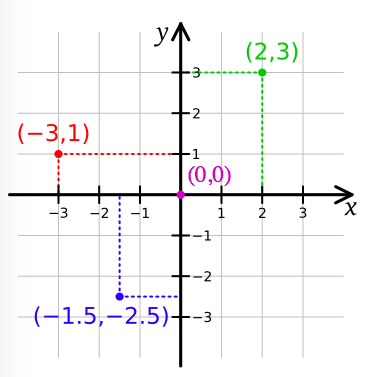
\includegraphics [scale=0.45] {coordinates.png} \end{center}

The first is to orient two number lines on a piece of paper, at right angles, and then consider pairs of numbers $(x,y)$ in the 2D plane.  Such pairs or tuples are called points.

Descartes published this idea in 1637.  The presentation would be difficult to recognize as our current system, but the germ is there:  axes where the position of a variable could be marked.  Only the positive numbers would be shown, and the axes not necessarily perpendicular.  As to the proofs, here is wikipedia on the subject:

\begin{quote}
His exposition style was far from clear, the material was not arranged in a systematic manner and he generally only gave indications of proofs, leaving many of the details to the reader.  His attitude toward writing is indicated by statements such as "I did not undertake to say everything," or "It already wearies me to write so much about it," that occur frequently. In conclusion, Descartes justifies his omissions and obscurities with the remark that much was deliberately omitted "in order to give others the pleasure of discovering [it] for themselves."
\end{quote}

The second idea of analytic geometry is to plot all the points that satisfy some mathematic relationship between $x$ and $y$, for example the parabola $y=x^2$.  

To do this, pick a few values of $x$ and calculate the corresponding values of $y$.  For example:  $(0,0), (\pm 1,1), (\pm 2, 4), \dots$.  Plot these points, and then finally, sketch the graph of the curve, without actually trying to plot \emph{all} of the individual points (of which there is an infinite number).  We make the assumption here that the function being plotted is continuous, so that the sketch of a curve between two points that are close enough together will be fairly smooth and for $x$-values close to the plotted $x$, have corresponding $y$-values not too different from the plotted $y$.

\subsection*{formulas for a line}

Suppose we pick two points $(x_1,y_1)$ and $(x_2,y_2)$, plot them on a graph, and then draw the line that connects them.  Recall Euclid's first two postulates:

$\circ$  A straight line segment can be drawn joining any two points.

$\circ$   Any straight line segment can be extended indefinitely in a straight line.
 
Now we want to derive an equation that describes (is valid for) all the points or pairs of values $(x,y)$ on this line.  A general approach is to say that the line has some slope $m$, which is defined as the rate of change of $y$, called $\Delta y$, divided by the rate of change of $x$:

\[ m = \frac{\Delta y}{\Delta x} = \frac{y_2 - y_1}{x_2 - x_1} \]

This is the \emph{point-slope equation}.

The value of $m$ might be zero, for a horizontal line, where all the values of $y$ are the same.  Or it might be undefined, for a vertical line, where all the values of $x$ are identical.  

In most cases, however, $m \ne 0$ and $m \in (-\infty, \infty)$.  That is, $|m|$ is not infinite but also non-zero.

Except in the case of the vertical line, we can write
\[ y = mx + b \]

for any two points $x$ and $y$ on a given line.  $b$ is called the $y$-intercept, it is the value of $y$ obtained when $x = 0$.  This is the \emph{slope-intercept equation} of the line.

Notice that the equation of a line is not determined just by the slope.  One can draw a whole family of parallel lines with the same slope and different $y$-intercepts.  For example here are three lines $y = 2x + b$ for $b = \{ 0, 1, 2 \}$.

\begin{center} 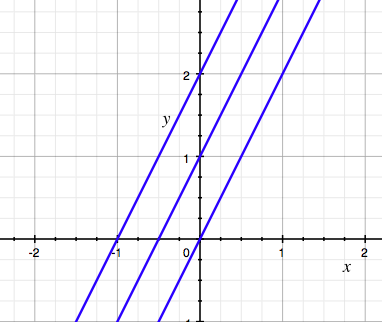
\includegraphics [scale=0.4] {line_family.png} \end{center}

The value of $x$ corresponding to $y = 0$ is the $x$ intercept
\[ x = -\frac{b}{m} \]

The first equation is easily derived from the second.  Plugging in specific values of $x$ and $y$ we have
\[ y_1 = mx_1 + b \]
\[ y_2 = mx_2 + b \]
Subtracting
\[ y_2 - y_1 = m(x_2 - x_1) \]
which rearranges to give the desired result.

\subsection*{formula for a circle}

A circle can be defined as all the points at the same distance from a central point, let us label that point $(h,k)$.  The distance from the points to the center is the radius, denoted $r$.

Using the Pythagorean theorem, we can calculate the square of the distance from the origin as
\[ r^2 = (x - h)^2 + (y - k)^2 \]

The simplest circles are those whose central point is the origin of the coordinate system.  In that case the equation  simplifies to 
\[ r^2 = x^2 + y^2 \]
Usually, we know the value of $r$ and we want to write an equation for $y$ in terms of $x$.  Then
\[ y^2 = r^2 - x^2 \]
\[ y = \sqrt{r^2 - x^2} \]

\subsection*{formula for a parabola}
A general formula for a parabola is
\[ y - y_0 = a(x - x_0)^2 \]
where $a$ is called the shape factor.  It governs how steeply the curve rises (and by its sign, in which direction it opens).

Multiplying out:
\[ y - y_0 = a(x^2 - 2xx_0 + x_0^2) \]
\[ y = ax^2 - 2ax_0 x + ax_0^2 + y_0 \]

In this form the cofactors are usually simplified as
\[ y = ax^2 + bx + c \]

Probably the most common problem with a quadratic equation like this is to find the roots, the values of $x$ for which $y=0$ is a solution.  These are the points where the graph of the curve crosses the $x$-axis (if it does so).
\[ ax^2 + bx + c = 0 \]

We can find a general formula for the solutions by the process of \emph{completing the square}.  First, multiply through by $1/a$ and rearrange:
\[ x^2 + \frac{b}{a} x = - \frac{c}{a} \]

The key insight is to recognize that if we add $(b/2a)^2$ to both sides, the left-hand side will become a perfect square:
\[ x^2 + \frac{b}{a} x + (\frac{b}{2a})^2 = -\frac{c}{a} + (\frac{b}{2a})^2 \]
\[ (x + \frac{b}{2a})^2 = -\frac{c}{a} + (\frac{b}{2a})^2 \]
\[ x + \frac{b}{2a} = \pm \sqrt{-\frac{c}{a} + (\frac{b}{2a})^2} \]

Multiplying top and bottom of the first term under the square root gives a common factor:
\[ x + \frac{b}{2a} = \pm \sqrt{-\frac{4ac}{4a^2} + (\frac{b}{2a})^2} \]
which can come out of the square root and then matches what's in the second term on the left-hand side:
\[ x + \frac{b}{2a} = \pm \frac{\sqrt{-4ac + b^2}}{2a} \]
which we rearrange slightly to give the standard \emph{quadratic formula}:
\[ x = \frac{-b \pm \sqrt{b^2 - 4ac}}{2a} \]

\subsection*{example}

Here is a moderately complicated figure we will see in a later chapter (\hyperref[sec:quad]{\textbf{here}}).

\begin{center} 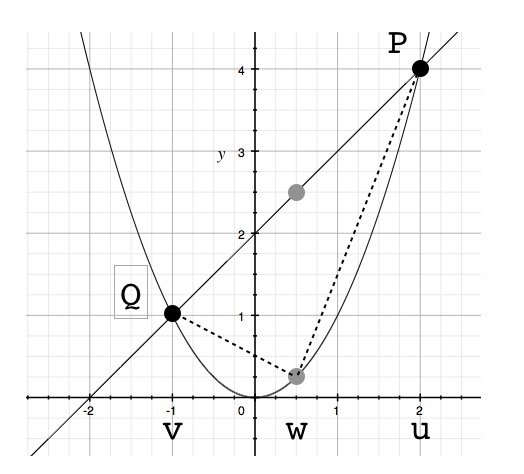
\includegraphics [scale=0.4] {para_tri2.png} \end{center}

It shows the two axes (horizontal and vertical lines with distances marked), and four points plotted plus a line, two line segments, and a parabola.  We can also "read" other points off the graph, such as the vertex of the parabola $(0,0)$, or the intersections of the line with the axes at $(-2,0)$ and $(0,2)$.

It is assumed you've studied analytic geometry before, so we won't say much more now than what is in this chapter.

A standard course in analytic geometry is concerned with the conic sections:  circle, ellipse, parabola and hyperbola.  Those are all wonderful topics, but we'll wait to explore them in detail in later chapters, where we can use a bit of calculus and also linear algebra.  

Nevertheless, we give an example in three parts as a taste of analytic geometry.

\subsection*{part 1}
Consider the simplest parabola:  $y = x^2$.

The point $(1,1)$ is on the curve, because $(x = 1, y = 1)$ satisfies the equation $y = x^2$.

\begin{center} 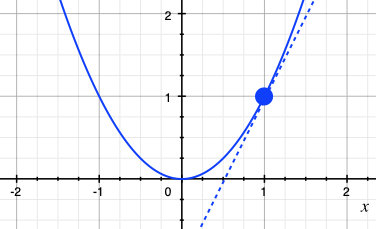
\includegraphics [scale=0.50] {para11.png} \end{center}

Suppose we know that the slope of the tangent to the curve at the point $(1,1)$ is equal to $2$.  (Using calculus this is trivial, we'll show a non-calculus method in the third example, below).  

The equation of the tangent line is
\[ y - y_0 = m(x - x_0) \]
\[ y - 1 = 2(x - 1) \]
\[ y = 2x - 1 \]

Now suppose that we knew only the parabola and this slope, but we did not know the point where the tangent meets the curve.  

We have the equation of a line:
\[ y = 2x + y_0 \]

We seek points which are simultaneously on the line and the curve.  They must satisfy both equations.

So, substitute for $y$ from the equation for the curve:
\[ x^2 = 2x + y_0 \]
\[ x^2 - 2x - y_0 = 0 \]

Now look at the quadratic formula we would use to solve this equation for $x$:
\[ x = \frac{-b \pm \sqrt{b^2 - 4ac}}{2a} \]

Since this is a tangent line, we seek the values for which this expression has only a single solution.  The tangent "kisses" the curve at a single point.

That will happen when the part under the square root (called the discriminant) is equal to zero.

\[ b^2 - 4ac = 0 \]
\[ b^2 = 4ac \]
\[ (-2)^2 = 4(- y_0) \]
\[ y_0 = -1 \]
So the equation of the tangent line is $y = 2x - 1$, as we had before.

In general, $y = 2x + y_0$ is a \emph{family} of lines.  For $y_0 = -1$, there is a single solution for $x$ to be both on the line and the parabola.  For $y_0 < -1$, there are no solutions, while for $y_0 > -1$ there are two solutions.

\subsection*{part 2}
Now suppose we have the same parabola and a point in the plane such as $(3,5)$.  We seek the equations of tangent lines to the parabola that go through this point.  
\begin{center} 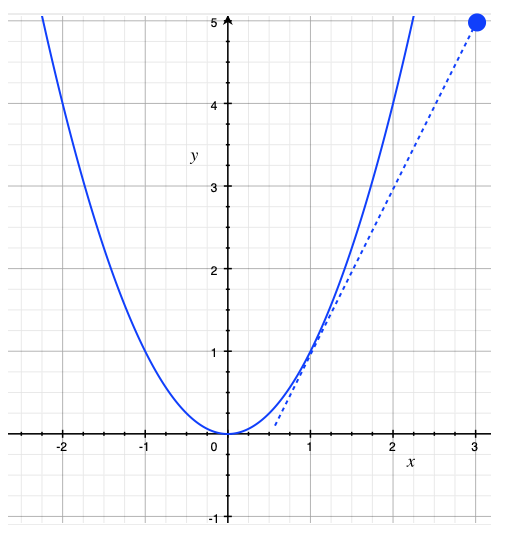
\includegraphics [scale=0.50] {para12.png} \end{center}

There will be two of them

The equations of lines passing through this point, with different slopes $m$ are given by:

\[ y - y_0 = m(x - x_0) \]
\[ y - 5 = m(x - 3) \]

Since values of $(x,y)$ are both on the line and the parabola
\[ x^2 - 5 = mx - 3m \]
\[ x^2 - mx + (3m - 5) = 0 \]

Solutions are given by the quadratic equation:
\[ x = \frac{m \pm \sqrt{(-m)^2 - 4(3m - 5)}}{2} \]

The value of the slope $m$ giving a single solution (zero discriminant) is:
\[ m^2 - 12m + 20 = 0 \]
\[ (m - 2)(m - 10) = 0 \]
\[ m = 2, \ \ \ m = 10 \]

We knew the first one already, because the point $(3,5)$ is on the line $y = 2x - 1$.  This is the tangent to the curve at $(1,1)$, which has slope $m = 2$.
\begin{center} 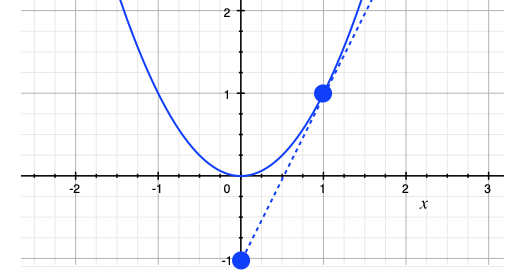
\includegraphics [scale=0.50] {para13.png} \end{center}

Actually, there is always another solution.  Any vertical line (with infinite slope) passes through only a single point on the parabola.

\subsection*{part 3}
Now suppose we have the same parabola and a point on it such as $(x_0,y_0)$.  

To find the equation of a tangent line through that point we need the slope $m$:
\[ y - y_0 = m(x - x_0) \]

To find points that satisfy both equations, plug in:
\[ x^2 - y_0 = m(x - x_0) \]
\[ x^2 - mx + (mx_0 - y_0) = 0 \]
Solve for $x$ using the quadratic equation.  

\[ x = \frac{m \pm \sqrt{m^2 - 4(mx_0 - y_0)}}{2} \]

Remember that we seek a slope where there is only a single $x$ that satisfies the equation.  Thus the discriminant should be zero.
\[ m^2 = 4(mx_0 - y_0) \]
\[ m^2 - 4mx_0 + 4y_0 = 0 \]

To find the slope, solve for $m$.  Again, using the quadratic, but we don't need to write the whole thing.  There is a unique tangent line, thus a unique slope.  Therefore, the discriminant should again be equal to zero.

That leaves, simply
\[ - \frac{b}{2a} = \frac{4x_0}{2} = 2 x_0 \]

The slope of the tangent line is $2x_0$ and in particular, at the point $(1,1)$ , the slope is equal to $2$.

If you work through this problem for a parabola with shape factor $a$, you will find that the equation for the slope is $m = 2ax_0$.

\subsection*{alternate solution}
\begin{center} 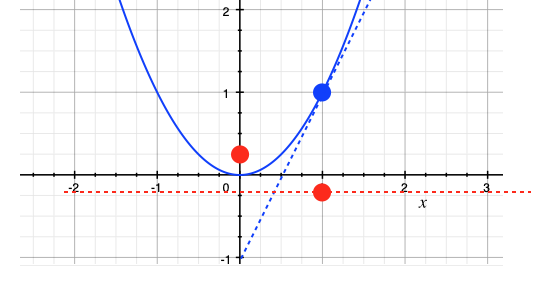
\includegraphics [scale=0.50] {para14.png} \end{center}

A parabola is defined geometrically by its focus, at the point $(p,0)$ for a centered parabola, paired with its directrix, which is the line $y = -p$ for a vertex at the origin.  

All points on the parabola lie at the same distance $d$ from the focus and the directrix.

A relatively advanced fact about the parabola is that any tangent line intersects the $y$-axis at the same distance $d$ from the focus.

\begin{center} 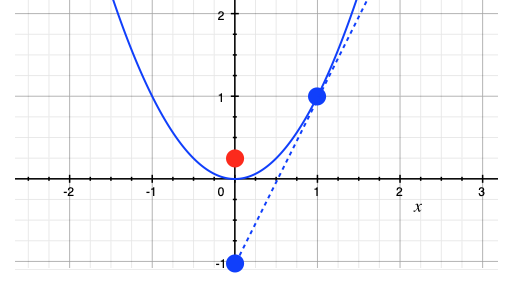
\includegraphics [scale=0.50] {para15.png} \end{center}

For $y = x^2$, consider the point $(x,x^2)$, and find the distance to the focus squared as 
\[ d^2 = (x)^2 + (x^2 - p)^2 \]
\[ d^2 = x^2 + x^4 - 2x^2p + p^2 \]

Call the $y$-intercept $y_0$ so then 
\[ y_0 + d = p \]
\[ d^2 = p^2 - 2py_0 + y_0^2 \]

Equating the two expressions:
\[ p^2 - 2py_0 + y_0^2 = x^2 + x^4 - 2x^2p + p^2 \]
\[ y_0^2 - 2py_0 = x^2(1 + x^2 - 2p)  \]

In this case, we know $x = 1$ and $p = 1/4$ so
\[ y_0^2 - \frac{y_0}{2} - (2 - \frac{1}{2}) = 0 \]

We factor to obtain:
\[ (y_0 + 1)(y_0 - \frac{3}{2}) = 0 \]

$y_0 = -1$ was our solution above.

[ ?? What is the significance of the other solution?? ]


\end{document}